% small.tex
\documentclass[aspectratio=169]{beamer}

\usetheme{Boadilla}
\usepackage{amsmath}
\usepackage{graphicx}
\usepackage{wrapfig}
%algorithms and pseudo code
\usepackage{algorithm}
\usepackage[noend]{algpseudocode}
\usepackage{numprint}
\usepackage{subcaption}
\usepackage{media9}
\usepackage{bibentry}
\usepackage[autoplay,loop]{animate}
\usepackage[justification=centering]{caption}
\nobibliography*

\setlength{\abovecaptionskip}{1pt}
\setlength{\belowcaptionskip}{-10pt}
\setlength{\leftmargini}{5pt}
\setlength{\leftmarginii}{10pt}
\setlength{\leftmarginiii}{15pt}

\usepackage{graphicx}

\setbeamertemplate{bibliography item}[text]
\setbeamertemplate{author in head/foot}{\insertshortauthor}
\setbeamertemplate{navigation symbols}{}

\newcommand{\lenitem}[2][.6\linewidth]{\parbox[t]{#1}{\strut #2\strut}}
\newcommand{\outline}{
  \begin{frame}<beamer>
    \frametitle{Outline}
    \tableofcontents[currentsection]
  \end{frame}
}

\newcommand{\outlinefull}{
  \begin{frame}<beamer>
    \frametitle{Outline}
    \tableofcontents
  \end{frame}
}

\begin{document}
\title[Partition Improvement for PIC]{

  MS60 Partitioning and Process Mapping for Emerging Architectures - Part II of II

  \textbf{Partition Improvement for High-Order Unstructured Mesh and Particle-In-Cell Simulations}
}

\author[G. Diamond]{\underline{Gerrett Diamond}, Cameron W. Smith, Mark S. Shephard}

\institute[SCOREC]{
  Scientific Computation Research Center \\
  Rensselaer Polytechnic Institute
}

\date{February 25, 2022}

%----------- titlepage ----------------------------------------------%
\begin{frame}[plain]
  \titlepage
\end{frame}

\outlinefull

\section{EnGPar: Diffusive Partition Improvement Tool}

\begin{frame}
  \frametitle{What is EnGPar?}
  \begin{itemize}
    \setlength\itemsep{1em}
  \item A partitioning tool to complement existing partitioning methods.
  \item Provides a diffusive load balancing algorithm for partition improvement with support for multi-criteria partitioning.
  \item Fast iterative algorithm permits usage during simulation runtime for dynamic load balancing.
  \item Utilizes a specialized multigraph structure to represent relation based data.
  \item Original methods designed for unstructured mesh simulations, but the usage of this graph structure allows for a broader range of applications.
  \item EnGPar's source can be found at \url{scorec.github.io/EnGPar}
  \end{itemize}
\end{frame}

\begin{frame}
  \frametitle{N-graph}
  \begin{columns}
    \begin{column}{.75\textwidth}
      \begin{itemize}
      \item Uses multi-hypergraph, N-graph, to represent user data with multiple types of relational connections:
        \begin{itemize}
        \item Vertices - Uniquely owned, represent partitioned data
        \item Hyperedges - Relational connections between sets of vertices
        \item $N$ sets of hyperedges represent different types of relations for multi-criteria
        \end{itemize}
      \item To map simulation data to the N-graph simulations:
        \begin{itemize}
        \item Define the partitioned units of work as the graph vertices.
        \item Define relationships between the units of work as hyperedges between the graph vertices.
        \item Additional types of relationships or criteria that require balancing are added as additional sets of hyperedges.
        \end{itemize}
      \end{itemize}
        \end{column}
    \begin{column}{.25\textwidth}
      \begin{figure}
        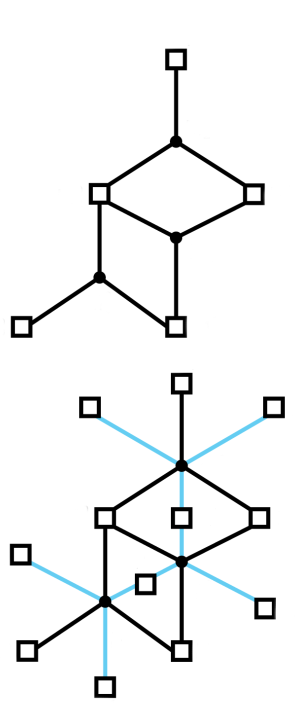
\includegraphics[height=.6\textheight]{examplegraphs.png}
        \caption*{Example N-graphs with one (top) and two (bottom) hyperedge types.}
      \end{figure}
    \end{column}
    \end{columns}
\end{frame}

\begin{frame}
  \frametitle{EnGPar - Diffusive Load Balancing Method}
  \begin{itemize}
  \item EnGPar takes as input a list of criteria (graph vertices or hyperedge types) and target imbalances for each criteria.
  \item The algorithm iteratively performs steps to improve the balance of one criteria at a time.
  \item In each iteration weight is diffused across part boundaries from highly loaded parts to lighter neighbors.
  \item The iterations are repeated until the criteria is satisfied or stagnation is detected.
  \item The next criteria is balanced with a new set of iterations maintaining the balance of previous criteria.
  \end{itemize}
\end{frame}

\section{Load Balancing High-Order Unstructured Mesh Simulations}
\outline

\begin{frame}
  \frametitle{High-Order Unstructured Mesh Case}
  \begin{itemize}
  \item Unstructured meshes coming from finite element/volume simulations are typically partitioned by:
    \begin{itemize}
    \item Elements - Element-Partitioned Mesh
    \item Vertices - Vertex-Partitioned Mesh
    \end{itemize}
  \item Costs associated with mesh entities are classified in two categories
    \begin{itemize}
    \item Computational - proportional to the number of mesh entities involved in the simulation computations.
    \item Communication - proportional to the number of shared mesh entities on the partition model boundary.
    \end{itemize}
  \item For high-order simulations, computational and communication costs are associated with multiple dimensions of mesh entity.
    \item Common mesh partitioning techniques (multilevel-graph/hypergraph and geometric) do not properly partition all mesh entities.
  \end{itemize}
\end{frame}

\begin{frame}
  \frametitle{N-graph for High-Order Unstructured Mesh}
  \begin{itemize}
  \item High-order experiments are run on an 3D element-partitioned mesh.
  \item Computation costs associated to all lower mesh-entity dimensions are represented.
  \item The N-graph is constructed with:
    \begin{itemize}
    \item Graph vertices constructed for each mesh element.
    \item Hyperedges constructed for each lower mesh entity.
    \item Two approaches to the sets of hyperedges are explored:
      \begin{enumerate}
      \item Hyperedge types for each lower mesh dimension (mesh vertices, mesh edges, mesh faces)
      \item One hyperedges type for all lower mesh entities.
      \end{enumerate}
    \end{itemize}
  \end{itemize}
  \begin{figure}
    \centering
    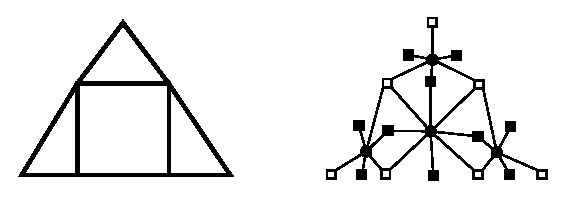
\includegraphics[height=.25\textheight]{meshToNgraphs.eps}
    \caption*{A 2D mesh (left) and N-graph (right) for element-partition with 2 hyperedge types for the mesh vertices (white squares) and mesh edges (black squares).}
  \end{figure}

\end{frame}

\begin{frame}
  \frametitle{High-Order Mesh Experiment}
  \begin{itemize}
    \item Problem Setup:
    \begin{itemize}
    \item 60 million mixed element mesh
    \item Global ParMETIS part k-way to 1Ki, 2Ki, 4Ki, and 8Ki parts
    \end{itemize}
    \item Hyperedges are weighted as follows:
      \begin{itemize}
      \item Mesh vertices have weight of 1
      \item Mesh edges have weight of 2
      \item Mesh triangles have weight of 1, Mesh quadrilaterals have weight of 2
      \end{itemize}
    \item Target reducing the total imbalance of the sum of hyperedge weights followed by the graph vertices.
    \item Experiments run on the Theta Supercomputer at Argonne
  \end{itemize}
\end{frame}

\begin{frame}
  \frametitle{High-Order Mesh - Imbalance}
  \begin{figure}[!ht]
    \centering
    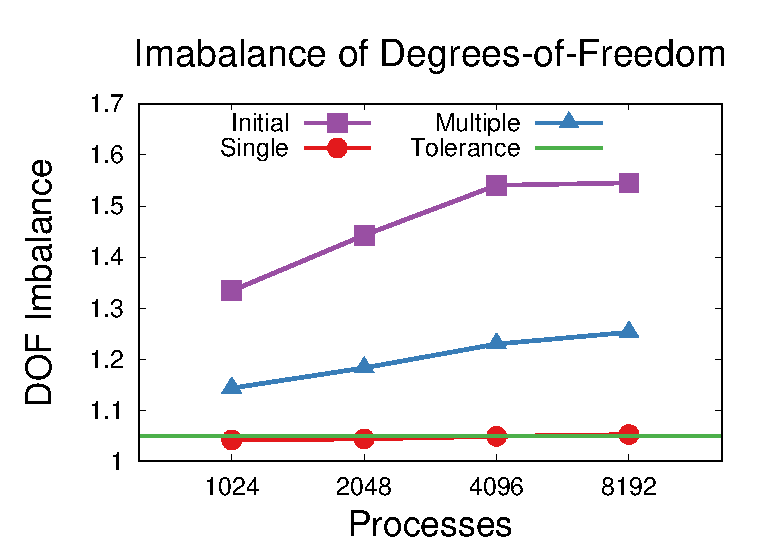
\includegraphics[width=.47\linewidth]{dof_v_cores.eps}
    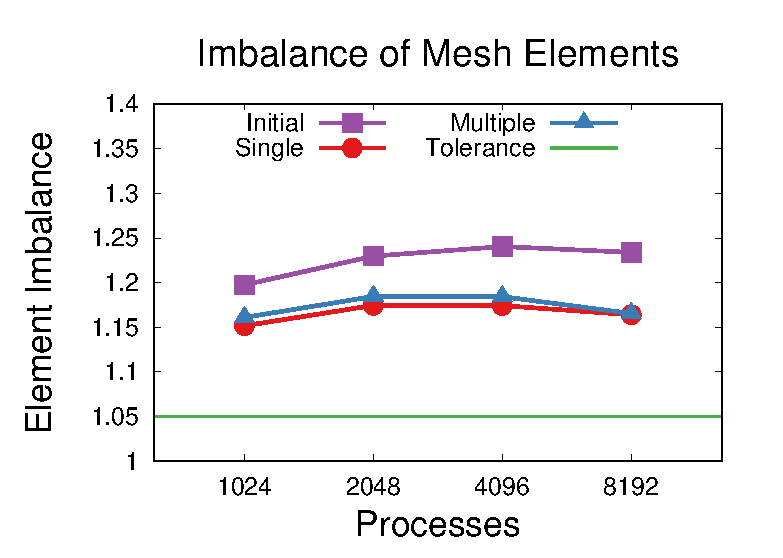
\includegraphics[width=.47\linewidth]{elm_v_cores.eps}
    \caption*{Imbalances of hyperedges (left) and graph vertices (right). \bf Lower is better}
  \end{figure}
  \vspace{.3cm}
  \begin{itemize}
  \item Single hyperedge type achieves a much lower imbalance of the hyperedges and slightly better for graph vertices.
  \item Single hyperedge iterations are more expensive than the multiple hyperedge case because the number of hyperedges traversed in each iteration is greater.
  \end{itemize}
\end{frame}

\section{Load Balancing for Particle-in-Cell Simulations}
\outline

\begin{frame}
  \frametitle{Unstructured Mesh Particle-In-Cell Simulations}
  \begin{itemize}
  \item Particle-In-Cell (PIC) simulations are time-advancing procedures that track particles as they move in a domain and interact with the governing fields.
  \item The domain is discretized using an unstructured mesh.
  \end{itemize}
  \begin{columns}
    \begin{column}{.6\linewidth}
      \begin{itemize}
      \item The general particle loop for a PIC application iterates over four steps:
        \begin{itemize}
        \item Particle Push - particle positions are updated based on mesh fields.
        \item Charge Deposition - based on the new particle positions, mesh fields are updated.
        \item Field Solve - domain level PDEs to update global mesh fields.
        \item Field-to-Particle - particle information is updated for the next push operation.
        \end{itemize}
      \end{itemize}
    \end{column}
    \begin{column}{.4\linewidth}
      \begin{figure}
        \centering
        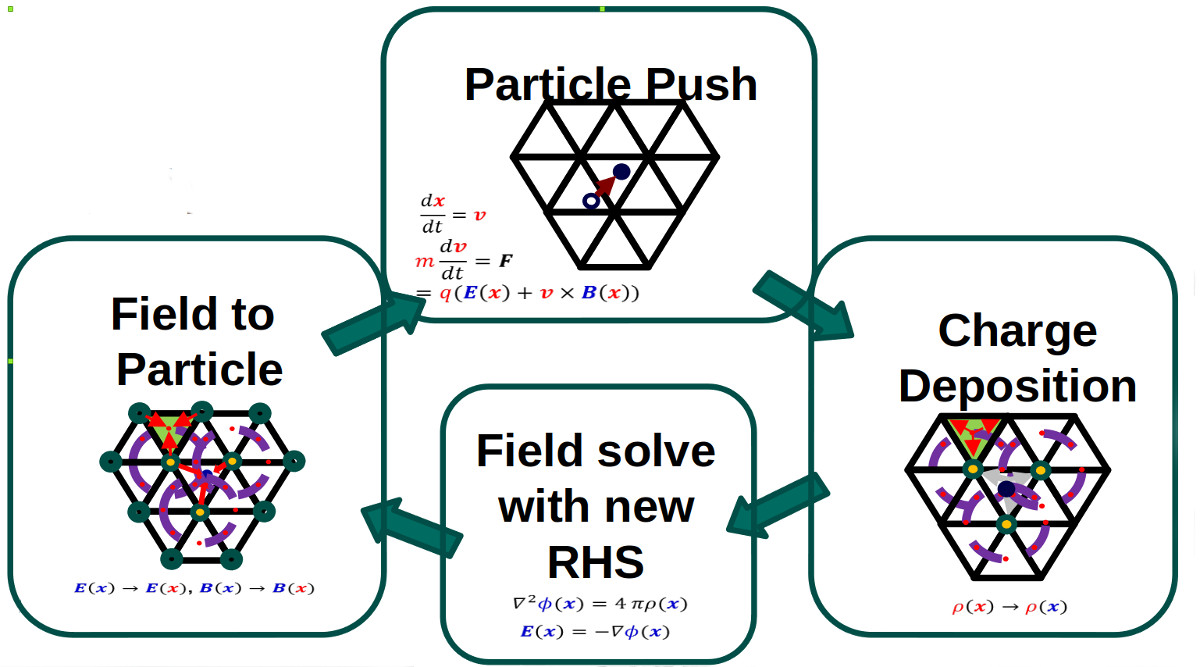
\includegraphics[width=.75\textwidth]{pic_loop.jpg}
        \caption*{Operations of PIC simulation's iteration loop}
      \end{figure}
    \end{column}
  \end{columns}
\end{frame}

%Mesh-based PIC + PICparts
\begin{frame}
  \frametitle{Approaches to PIC}
  \begin{itemize}
  \item Traditional approach to PIC is to primarily store particles
    \begin{itemize}
    \item Particles maintain knowledge of the mesh element it is within (parent element).
    \item A full copy of the mesh is maintained on all processes.
    \item Particles are distributed across processes
    \item Scalable wrt number of particles but not wrt mesh.
    \end{itemize}

  \item Mesh-based approach to PIC simulation store particles based on the parent mesh element:
    \begin{itemize}
    \item Particles are stored in memory based on their parent element.
      \begin{itemize}
      \item Easier to maintain a distributed mesh
      \end{itemize}
    \item Both particles and the mesh are distributed across processes
    \item Scalabale wrt number of particles and mesh entities.
    \end{itemize}
  \end{itemize}
\end{frame}

%Describe N-graph for PICparts and how to balance
\begin{frame}{Dynamic Load Balancing of Particles in Mesh-Based PIC}
  \begin{columns}
    \begin{column}{0.7\linewidth}
      \begin{itemize}
      \item To reduce communications the mesh partition is supplemented with sufficient buffering of nearby part's mesh entities.
      \item Each processes owned mesh entities plus the buffered entities make up a PICpart.
      \item A subset of the elements in a PICpart are denoted as safe for particles to be stored and operated on.
        \begin{itemize}
        \item If a particles moves to an unsafe element, then it must be migrated to a different process.
        \item Since there is overlap of the safe elements across processes there is an opportunity to migrate additional particles from a safe process to another safe process.
        \end{itemize}
      \end{itemize}
    \end{column}
    \begin{column}{0.3\linewidth}
      \begin{figure}
        \centering
        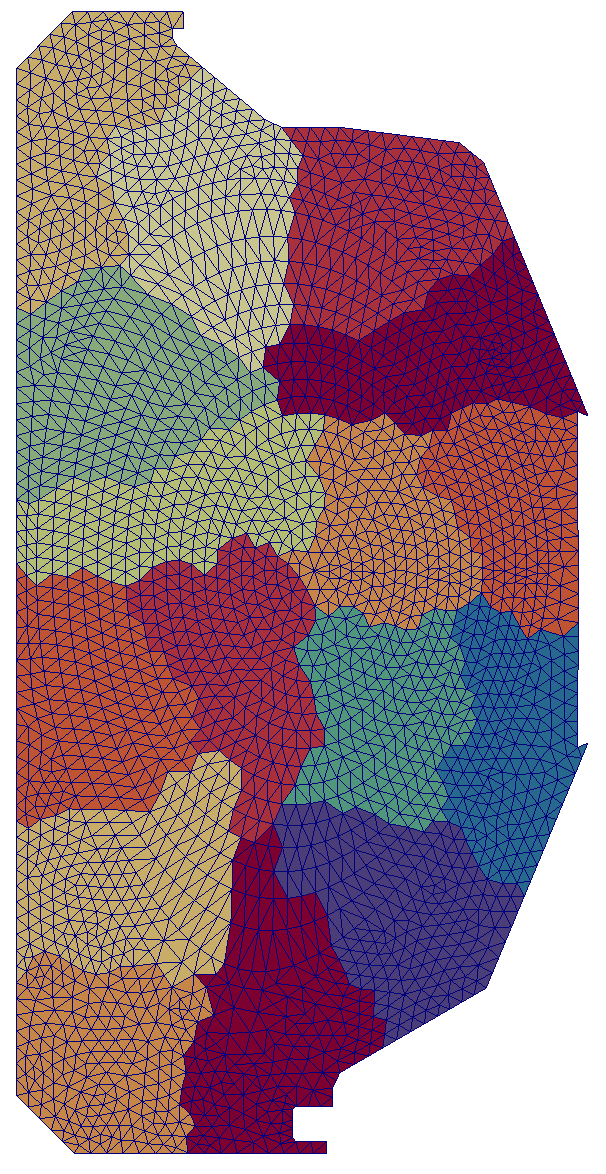
\includegraphics[height=.35\textheight]{xgcm_partition.png}
        \caption*{Partition of 2D mesh}
      \end{figure}
      \vspace{-.25cm}
      \begin{figure}
        \centering
        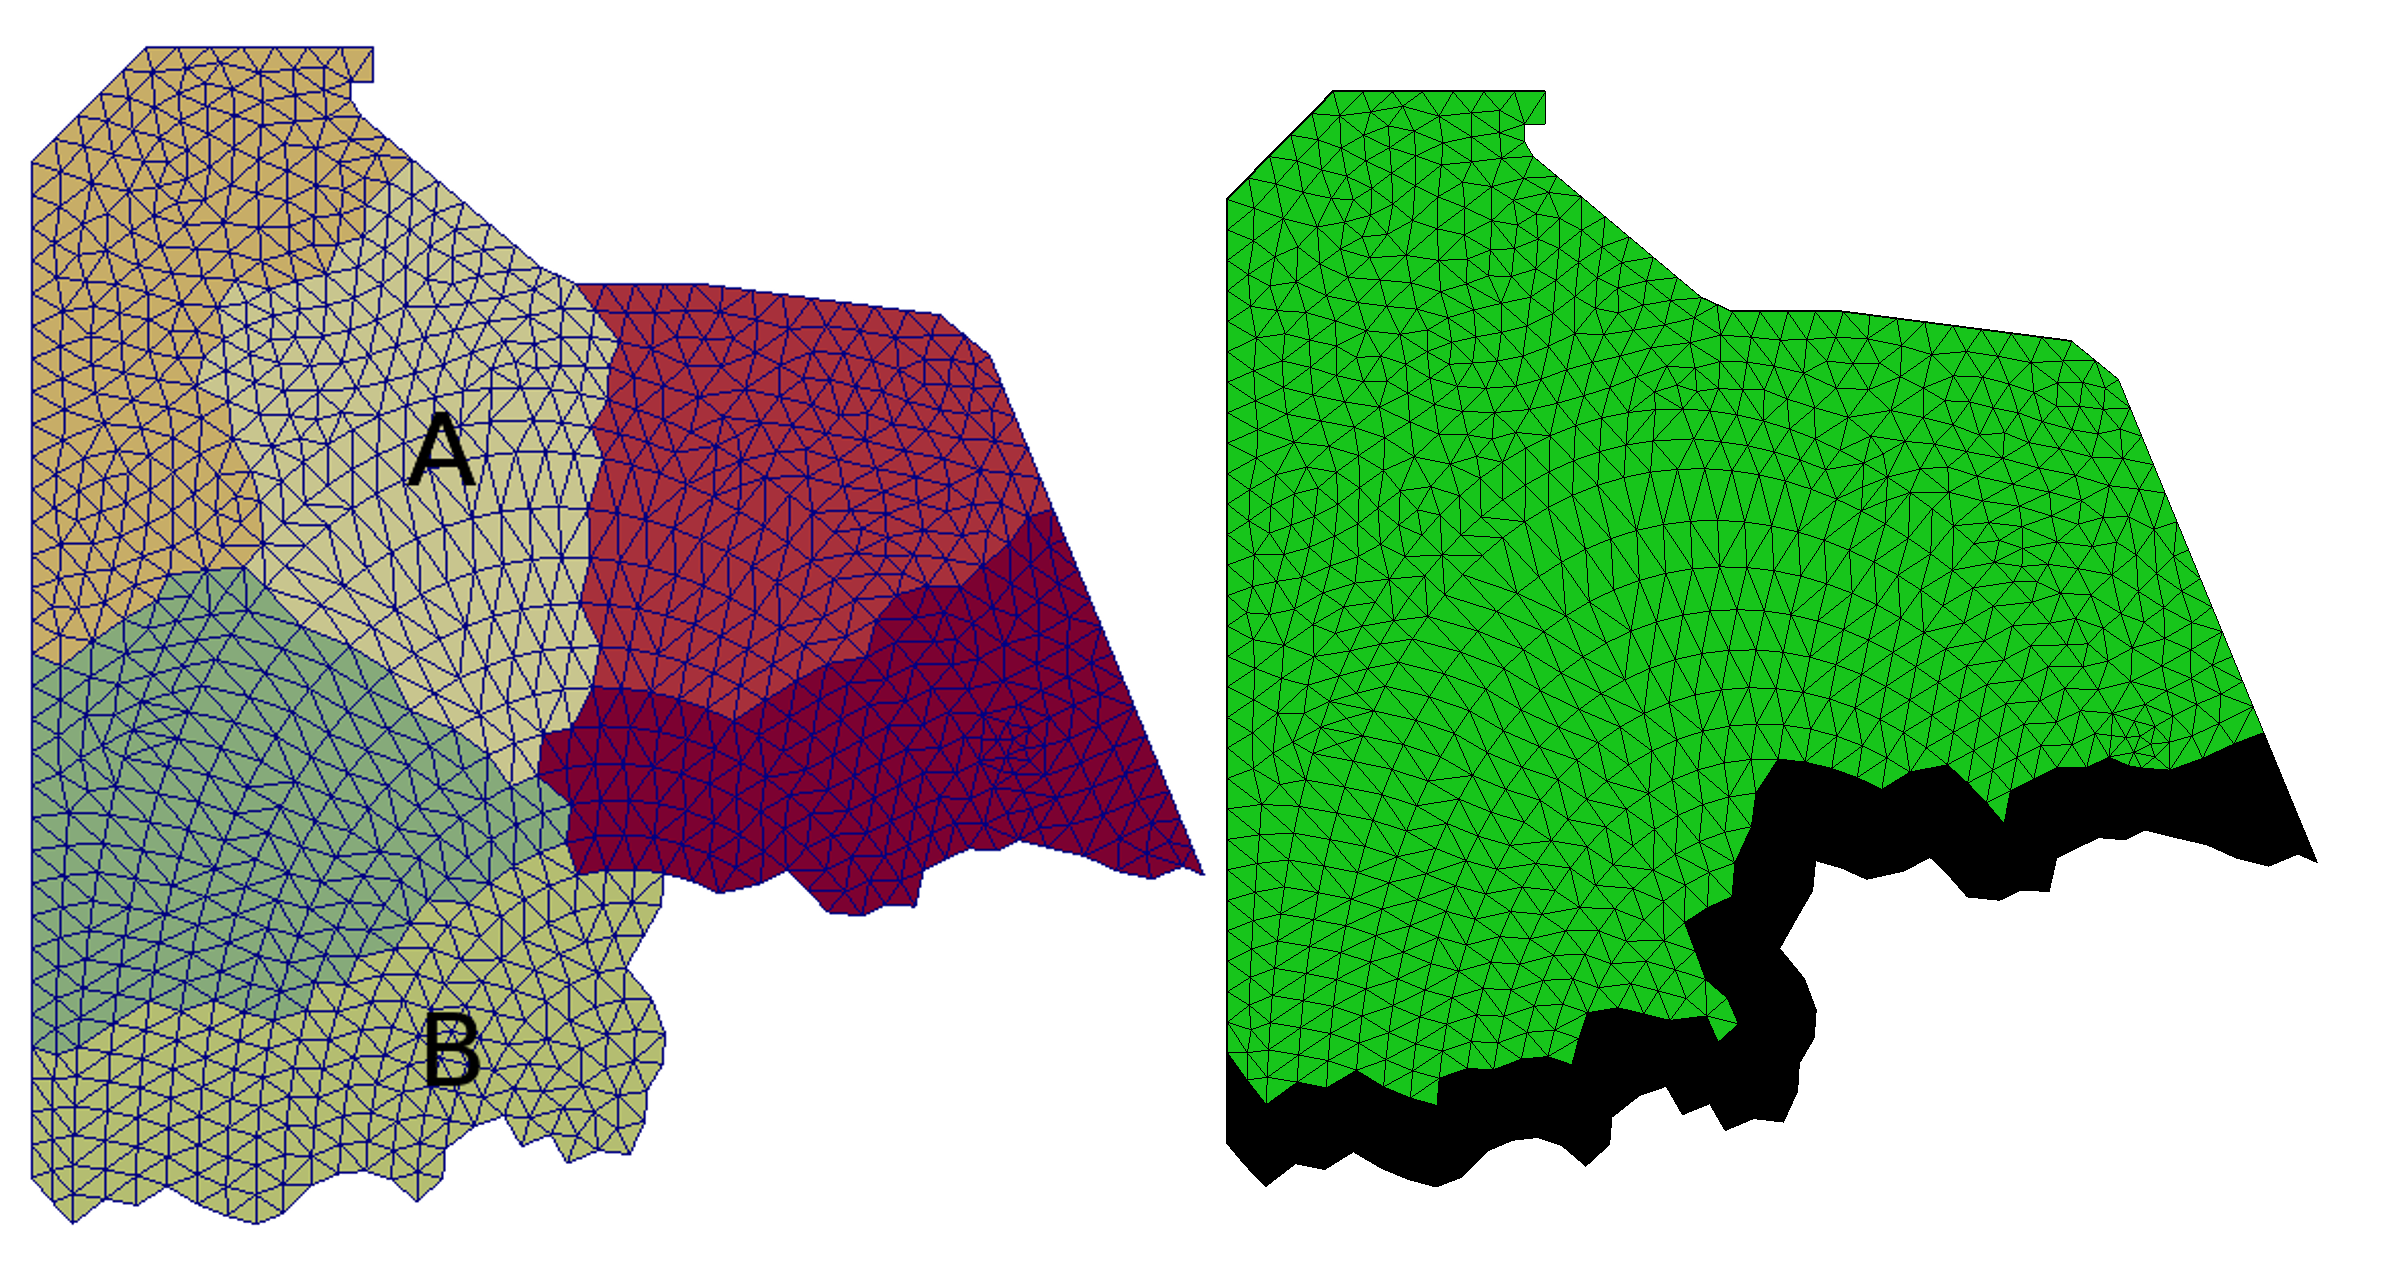
\includegraphics[width=\textwidth]{picpart.png}
        \caption*{PICpart for part A (left) and its safe zone (right)}
      \end{figure}
    \end{column}
  \end{columns}

\end{frame}


\begin{frame}{Overlapping Safe Zones}
  \begin{columns}
    \begin{column}{.5\textwidth}
      \begin{itemize}
      \item To determine where particles can migrate to, we introduce the notion of overlapping safe zones.
      \item For a set of PICparts $P$, the overlapping safe zone, $\bar{S}_P$, is the set of mesh elements such that each element is safe on each PICpart in $P$.
      \item The overlapping safe zones are constructed such that every mesh element belongs to exactly one $\bar{S}_P$.
        \begin{itemize}
        \item Some overlapping safe zones may be defined on one PICpart.
        \end{itemize}
      \item Any particle in an element in $\bar{S}_P$ can be migrated to any PICpart in $P$.
      \end{itemize}
    \end{column}
    \begin{column}{.5\textwidth}
      \begin{figure}
        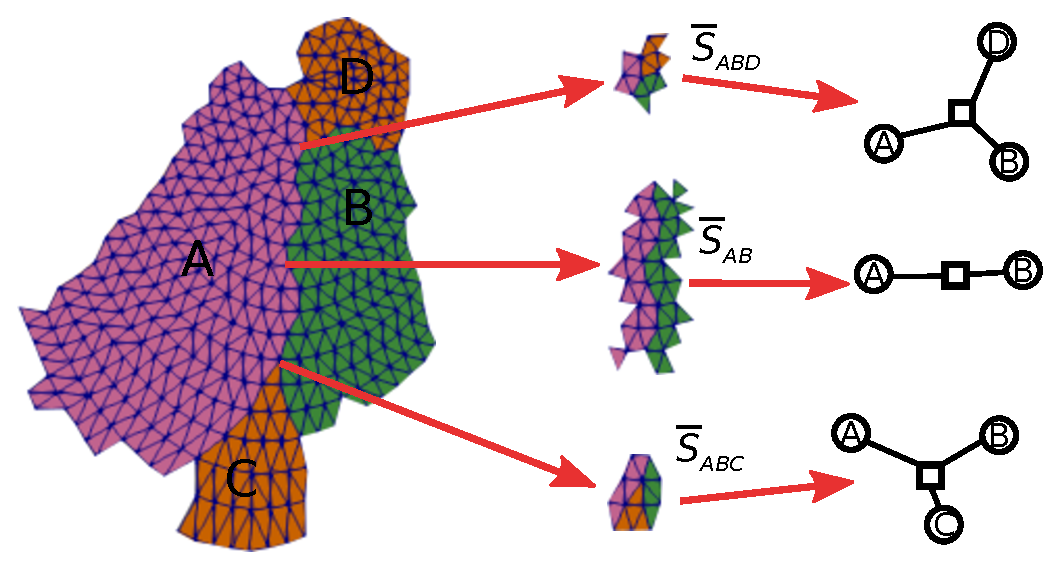
\includegraphics[width=.95\textwidth]{picpart_lb_new.eps}
        \caption*{Four cores (left) with three $\bar{S}_P$(right) on the boundary between cores A and B.}
      \end{figure}
    \end{column}
  \end{columns}
\end{frame}

\begin{frame}{Overlaping Safe Zones}
  \begin{columns}
    \begin{column}{.5\textwidth}
      \begin{itemize}
      \item We construct a hypergraph based on the overlapping safe zones as follows:
        \begin{itemize}
        \item For each $\bar{S}_P$ a subhypergraph is constructed.
        \item In the subhypergraph, one graph vertex is made for each PICpart in $P$.
        \item Each graph vertex in the subhypergraph is connected by one hyperedge for the $\bar{S}_P$.
        \end{itemize}
      \item The size of the hypergraph is significantly smaller than the original mesh as seen in the example table below.
      \end{itemize}
    \end{column}
    \begin{column}{.5\textwidth}
      \begin{figure}
        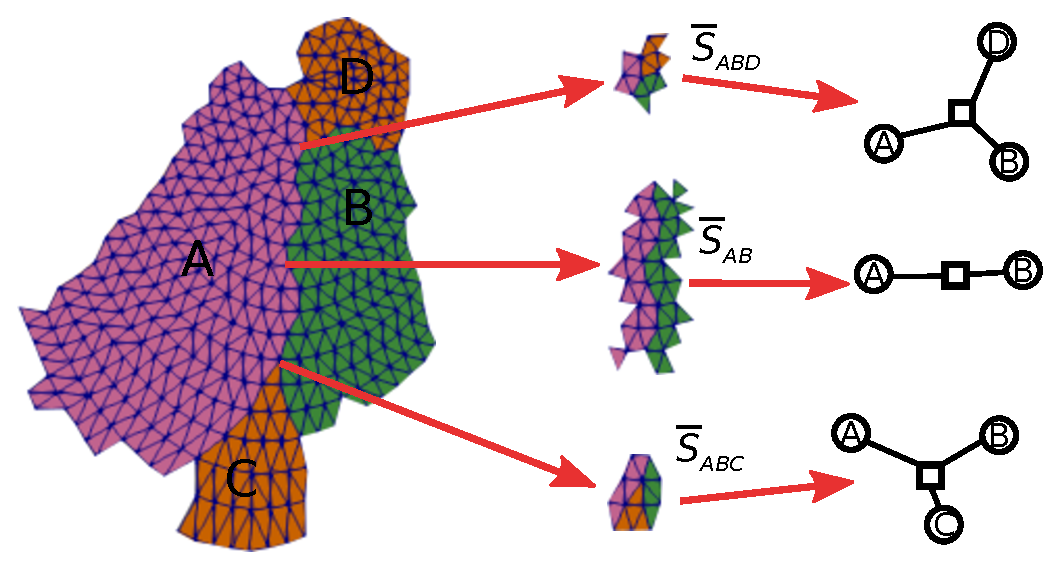
\includegraphics[width=.95\textwidth]{picpart_lb_new.eps}
        \caption*{Three $\bar{S}_P$(middle) on the boundary of cores A and B and corresponding subhypergraphs(right).}
      \end{figure}
    \end{column}
  \end{columns}
  \begin{table}
    \caption*{PICpart vs Hypergraph sizes for 11.4 million element mesh}
    \vspace{.1in}
    \begin{tabular}{|c|c|c|c|c|}
      \hline
      Number of PICparts & 6 & 12 & 24 & 48 \\
      \hline
      Average Elements per PICpart & 8.8M & 5.3M & 3.7M & 2.3M\\
      \hline
      Total Graph Vertices & 20 & 102 & 450 & 1931 \\
      \hline
      Total Graph Hyperedges & 3 & 19 & 69 & 266 \\
      \hline
    \end{tabular}
  \end{table}
\end{frame}

\begin{frame}{Diffusive Load Balancing with EnGPar}
  %Introduce EnGPar
  \begin{itemize}
    %Discuss how diffusive load balancing easily maps to this problem
  \item Applying EnGPar to our graph of overlapping safe zones
    \begin{itemize}
    \item Treat particles as contributions to the weight on each graph vertex.
    \item Weight is diffused between vertices across hyperedges.
    \item EnGPar creates a plan defining how much weight to send from process to process per hyperedge.
    \end{itemize}
  \end{itemize}
  Steps to perform load balancing with EnGPar
  \begin{enumerate}
    %Discuss the weighting of the graph
  \item Apply the number of particles in each $\bar{S}$ on each PICpart as the weight of the corresponding graph vertex.
  \item Run EnGPar's weight load balancer on the hypergraph to produce migration plan.
  \item Select particles to satisfy the plan from EnGPar.
  \end{enumerate}
\end{frame}

%Introduce GITRm example
\begin{frame}
  \frametitle{GITRm Experiments}
  \begin{itemize}
  \item Experiments performed on RPI's AiMOS supercomputer.
    \begin{itemize}
    \item Each Node has six NVIDIA Tesla V100 with 32GiB of memory.
    \item One MPI process per GPU.
    \end{itemize}
  \item Performance studies performed on GITRm
    \begin{itemize}
    \item Particles start at the bottom region of the domain.
    \item Particles curve around the domain moving upwards.
    \end{itemize}
  \item 11.4 million element mesh distributed up to 48 ranks.
  \item 25 million to 400 million particles simulated.
  \item 10,000 iterations performed with load balancing every 100 iterations.
  \end{itemize}
  \begin{figure}
    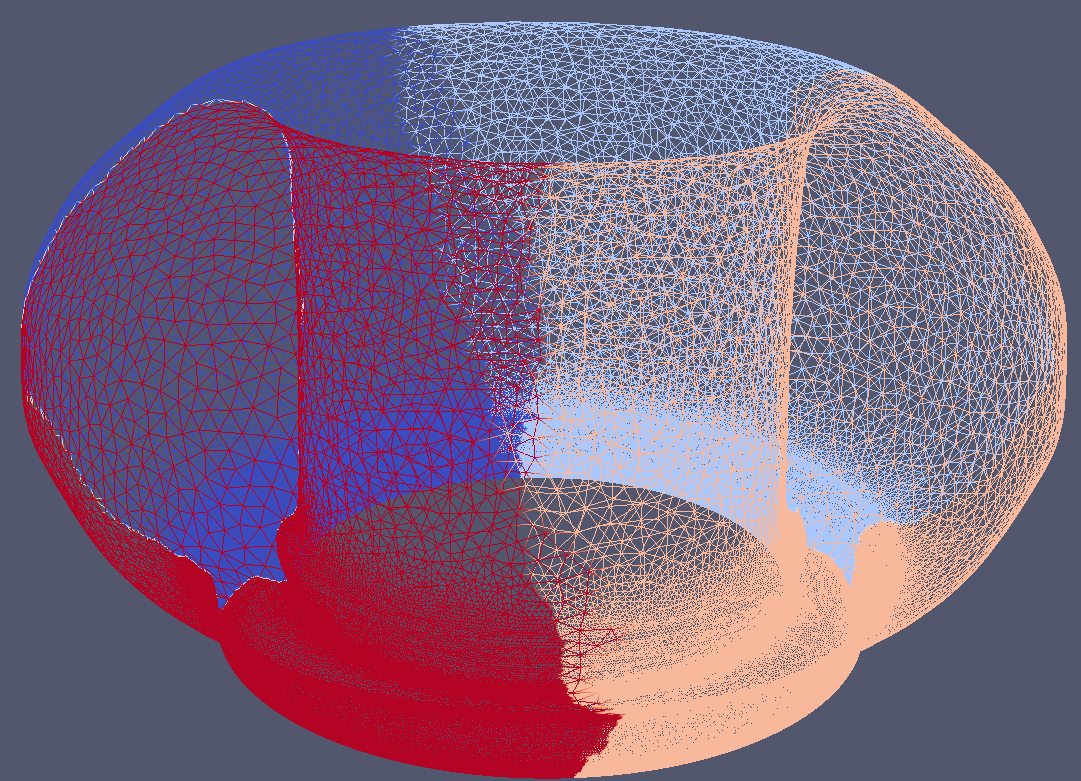
\includegraphics[height=.3\textheight]{gitrm_part_4.png}
    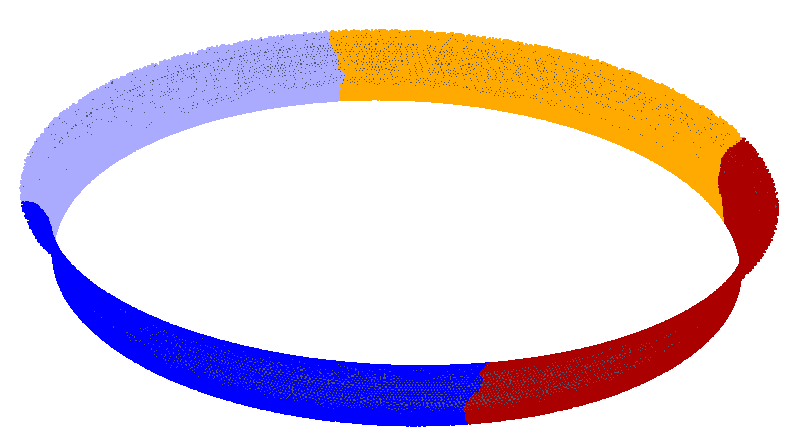
\includegraphics[height=.3\textheight]{gitrm_ptcl_init.png}
    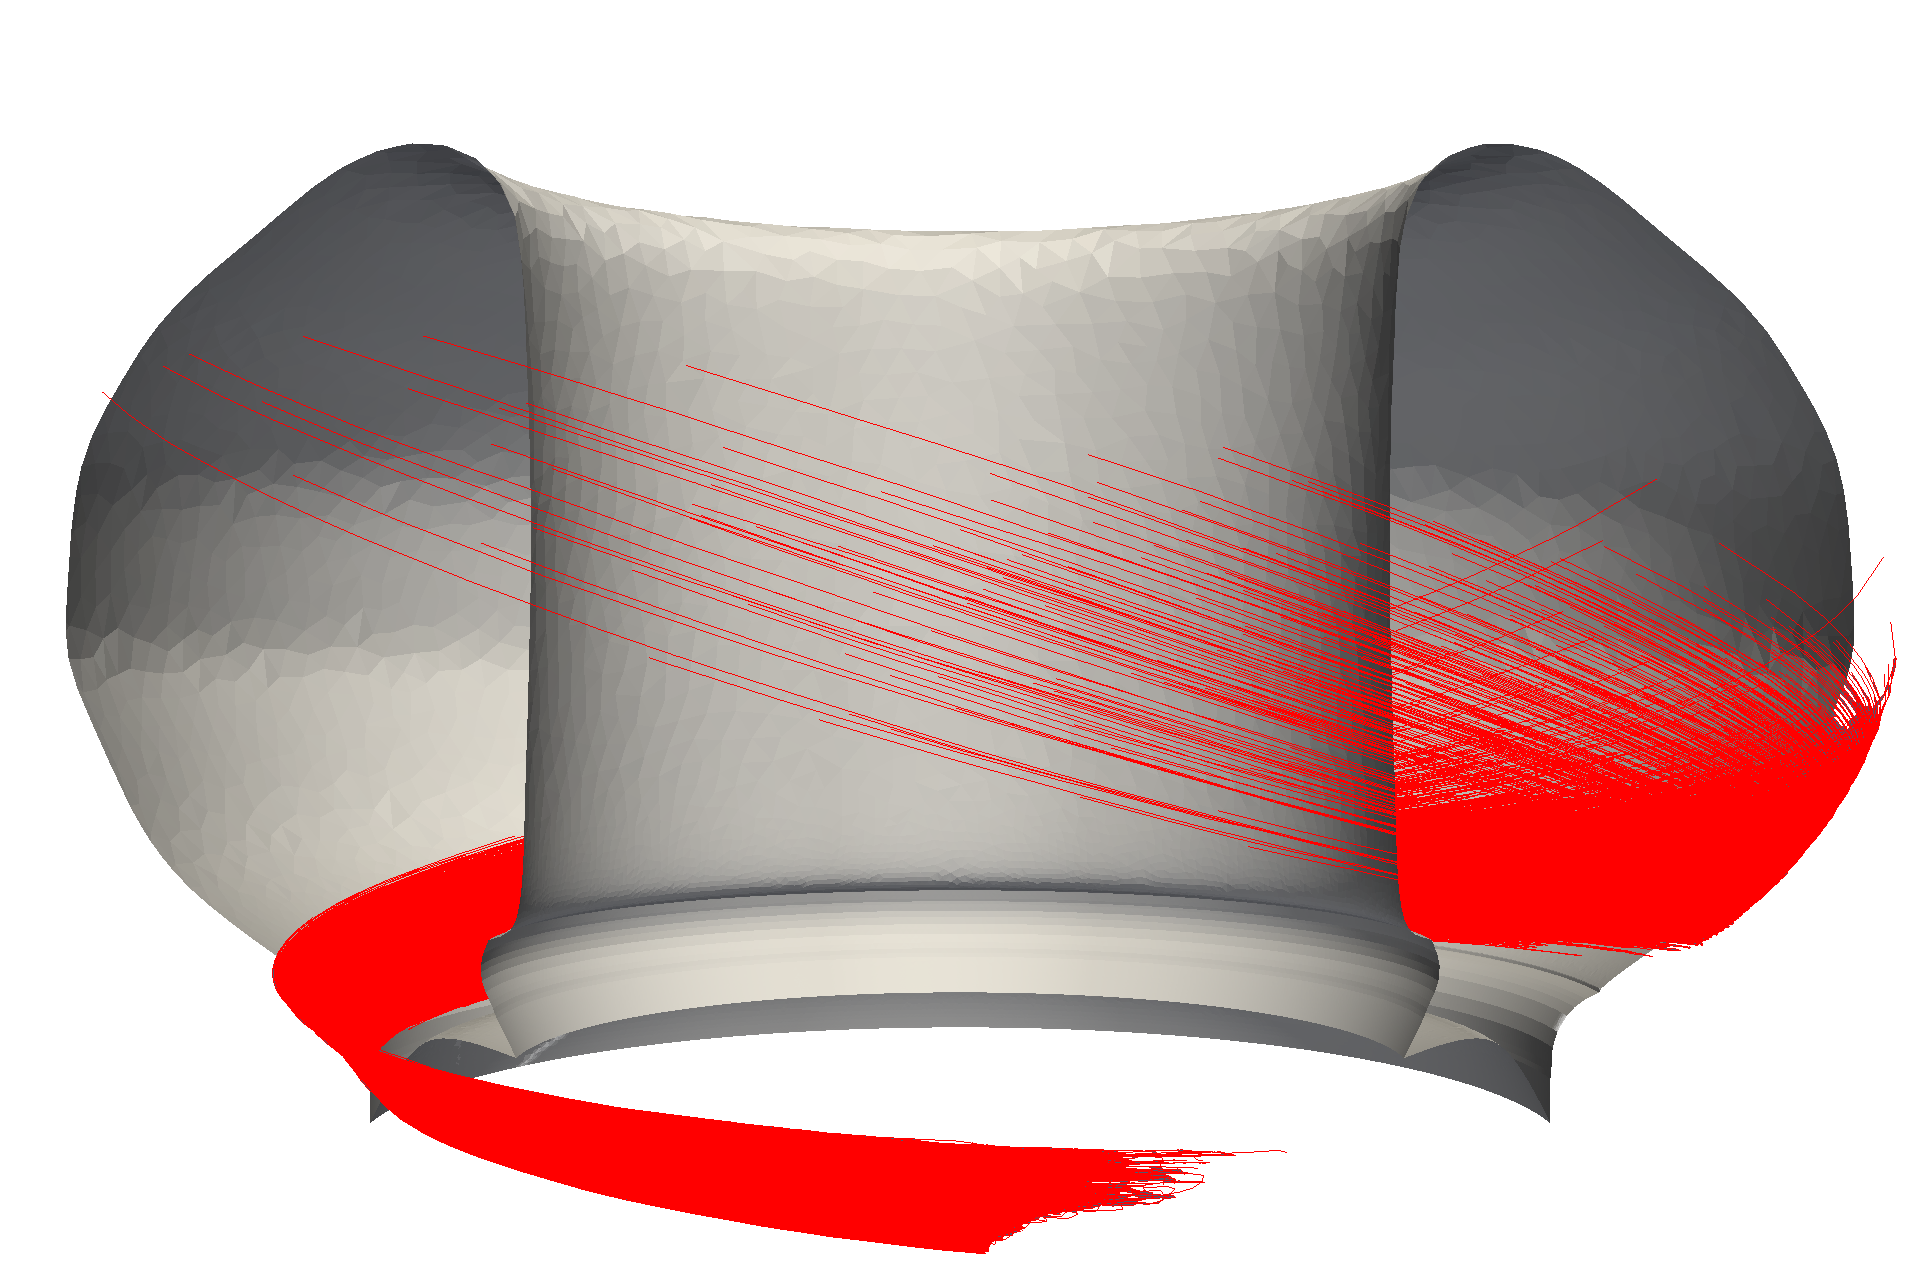
\includegraphics[height=.3\textheight]{gitrm_ptcl_movement.png}
    \caption*{Partitioned mesh, elements with particles at iteration 0, trajectories of some particles}
  \end{figure}
\end{frame}

% Show results + summary
\begin{frame}
  \frametitle{GITRm Particle Imbalance Results}
  %Report no lb vs lb timing of full simulation
  %Show 3-6 plots of lb for different cases
  \begin{figure}
    \centering
    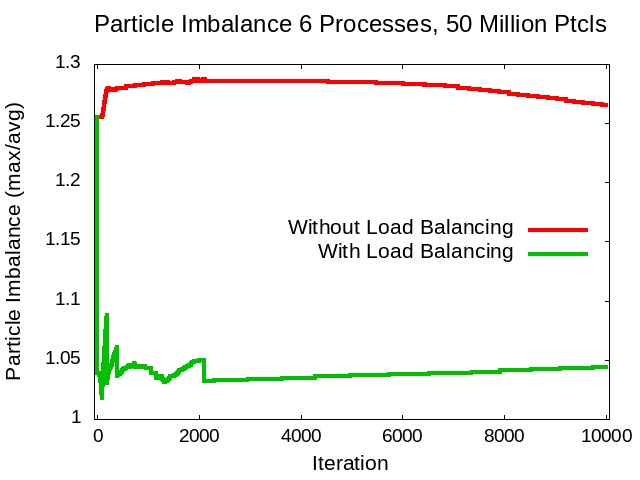
\includegraphics[width=.24\textwidth]{gitrm_imb_50m_6p.png}
    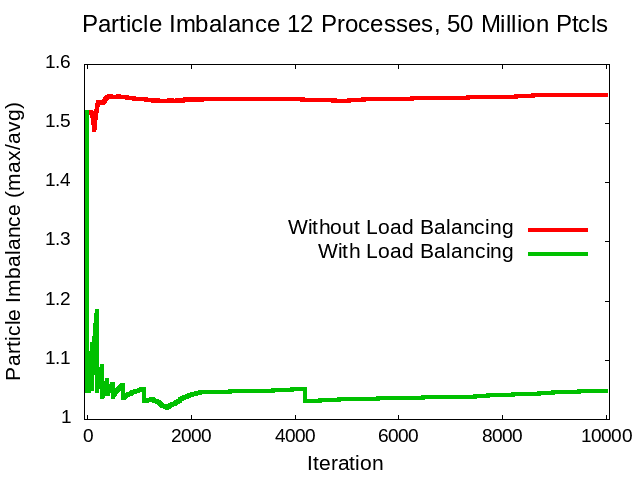
\includegraphics[width=.24\textwidth]{gitrm_imb_50m_12p.png}
    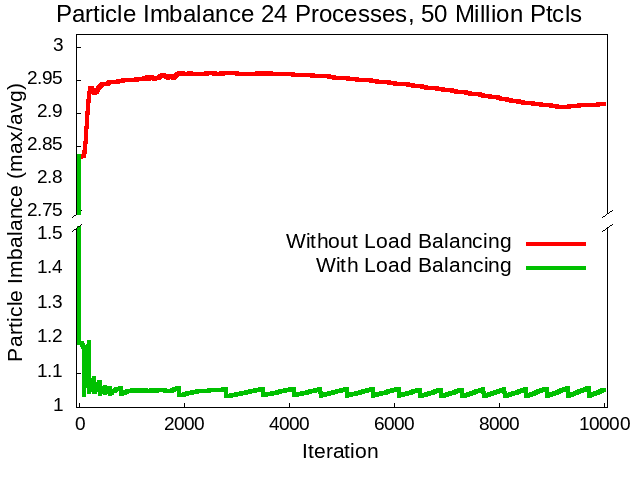
\includegraphics[width=.24\textwidth]{gitrm_imb_50m_24p.png}
    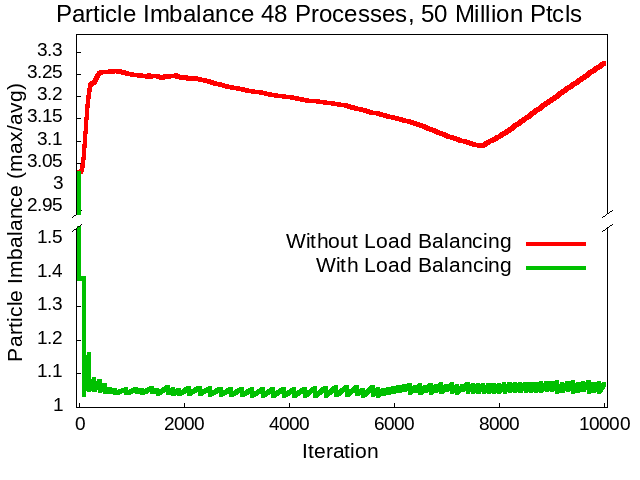
\includegraphics[width=.24\textwidth]{gitrm_imb_50m_48p.png}
  \end{figure}
  \vspace{-.25in}
  \begin{figure}
    \centering
    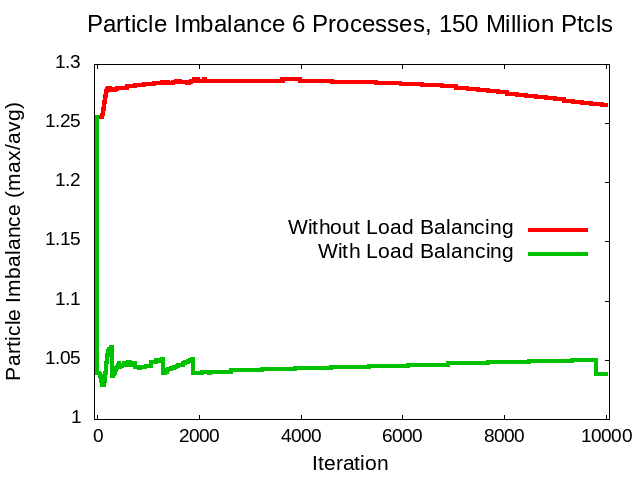
\includegraphics[width=.24\textwidth]{gitrm_imb_150m_6p.png}
    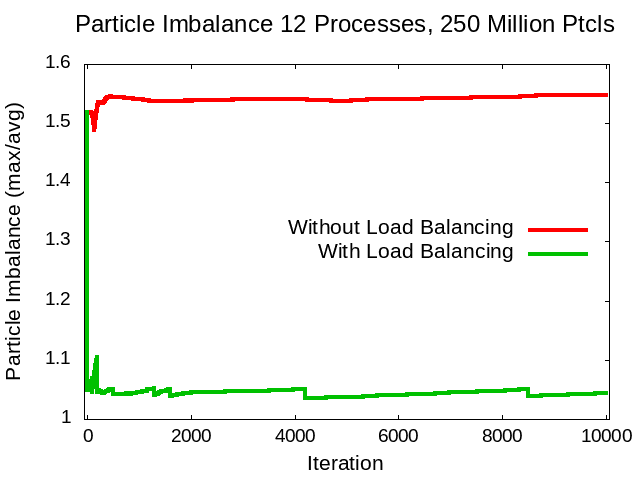
\includegraphics[width=.24\textwidth]{gitrm_imb_250m_12p.png}
    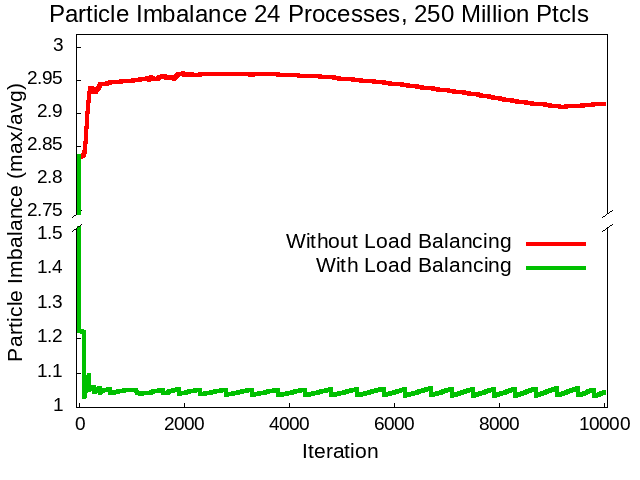
\includegraphics[width=.24\textwidth]{gitrm_imb_250m_24p.png}
    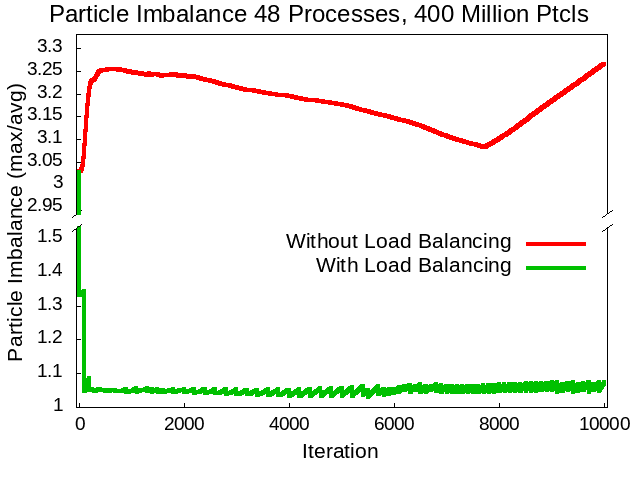
\includegraphics[width=.24\textwidth]{gitrm_imb_400m_48p.png}
    \caption*{Various GITRm setups executed with and without load balancing. \bf Lower is better}
  \end{figure}
  \begin{itemize}
  \item Particles are balanced below 5\% within the first few load balance exectutions.
  \item Particle imbalance is maintained after initial dispersion of particles
  \end{itemize}
\end{frame}


\begin{frame}
  \frametitle{GITRm Timing Summary}
  \begin{itemize}
  \item Performing load balancing took on average .04\% of the particle loop time.
  \item At most load balancing took .07\% of the particle loop time with 25 million particles on  48 processes.
  \item Speedups of up to 20\% were achieved when running load balancing.
  \item When the number of particles per GPU is low, using load balancing results in a slowdown due to increase communications without any speedup in computation.
  \item Ongoing research into which operations are speeding up or slowing down as a result of load balancing the particles.
  \end{itemize}
\end{frame}

%Introduce XGC partitioning requirements
\begin{frame}
  \frametitle{Traditional PIC simulation: XGC}
  \begin{columns}
    \begin{column}{.7\textwidth}
      \begin{itemize}
      \item In XGC, a copy of the 2D unstructured mesh is maintained on each process.
      \item The third spatial dimension is implicitly simulated by copies of the plane around the toroidal domain.
      \item Particles and operations performed on the mesh for each plane are partitioned
        across processes.
      \item The mesh is partitioned by a 1D partition of the mesh vertices
        \begin{itemize}
        \item $[0, N_0) \rightarrow$ process 0, $[N_0, N_1) \rightarrow$ process 1, etc.
        \end{itemize}
      \item The current approach to load balancing specifically targets three major components of the simualtion:
        \begin{itemize}
        \item Electron particles
        \item Ion particles
        \item The most expensive mesh operation: the collision operator.
        \end{itemize}
      \item Current load balancing algorithm in XGC is specificly targeting these three criteria.
      \end{itemize}
    \end{column}

    \begin{column}{.3\textwidth}
      %TODO: Generate better image of mesh
      \begin{figure}
        \centering
        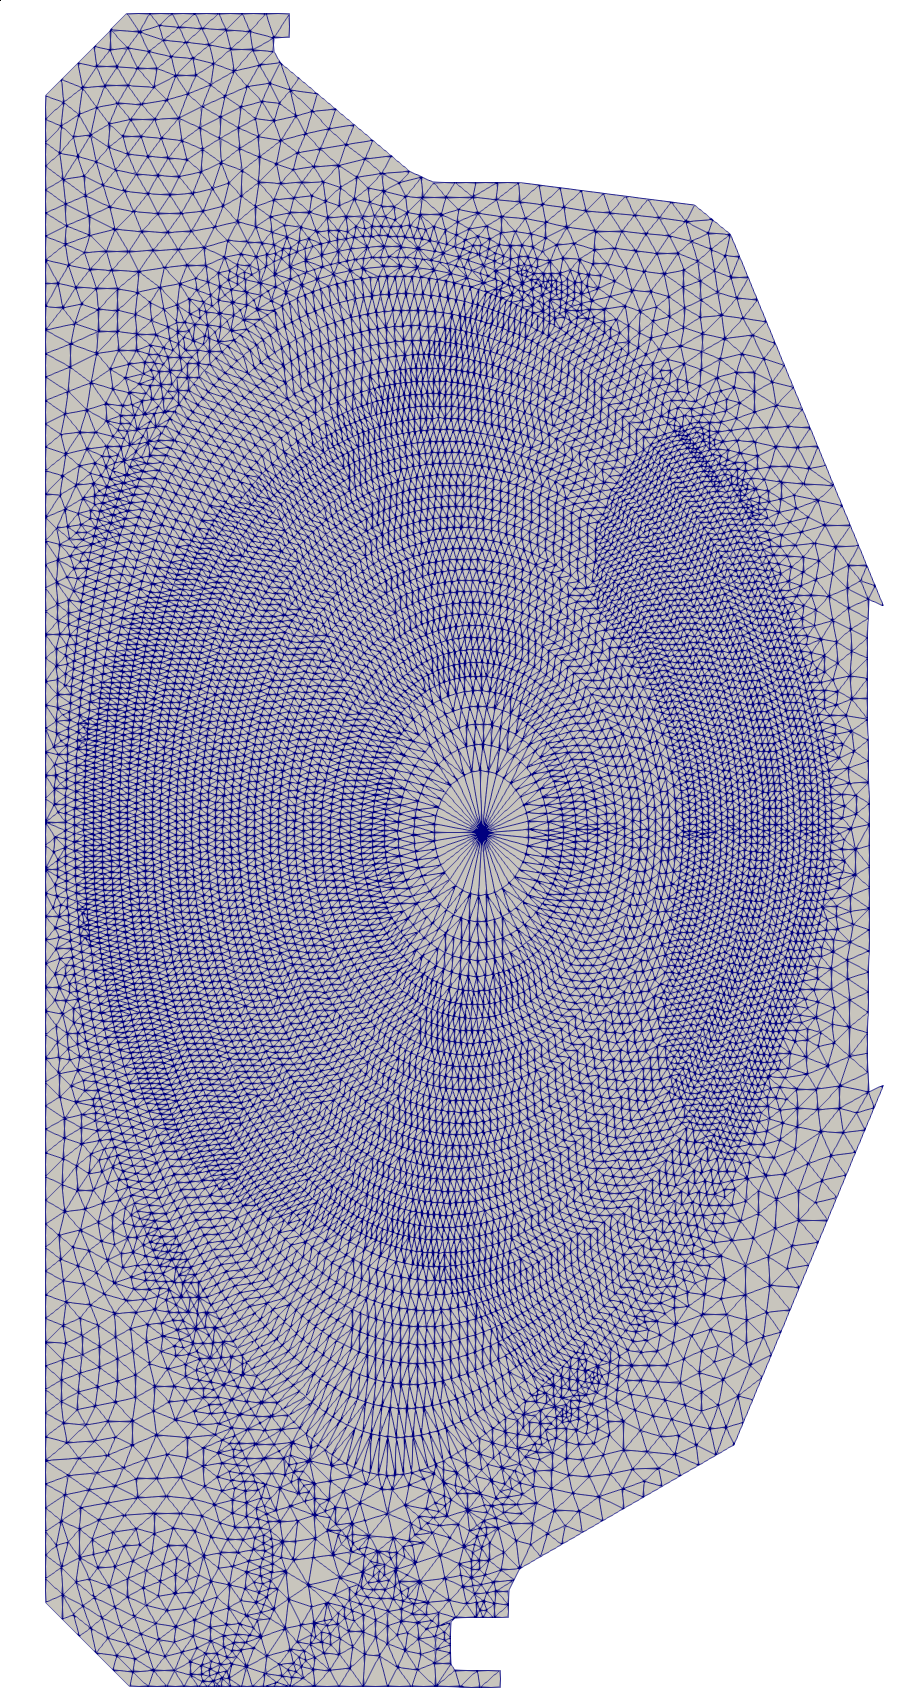
\includegraphics[height=.35\textheight]{itg24k.png}
        \caption*{2D mesh of the plane}
      \end{figure}
      \vspace{-.25cm}
      \begin{figure}
        \centering
        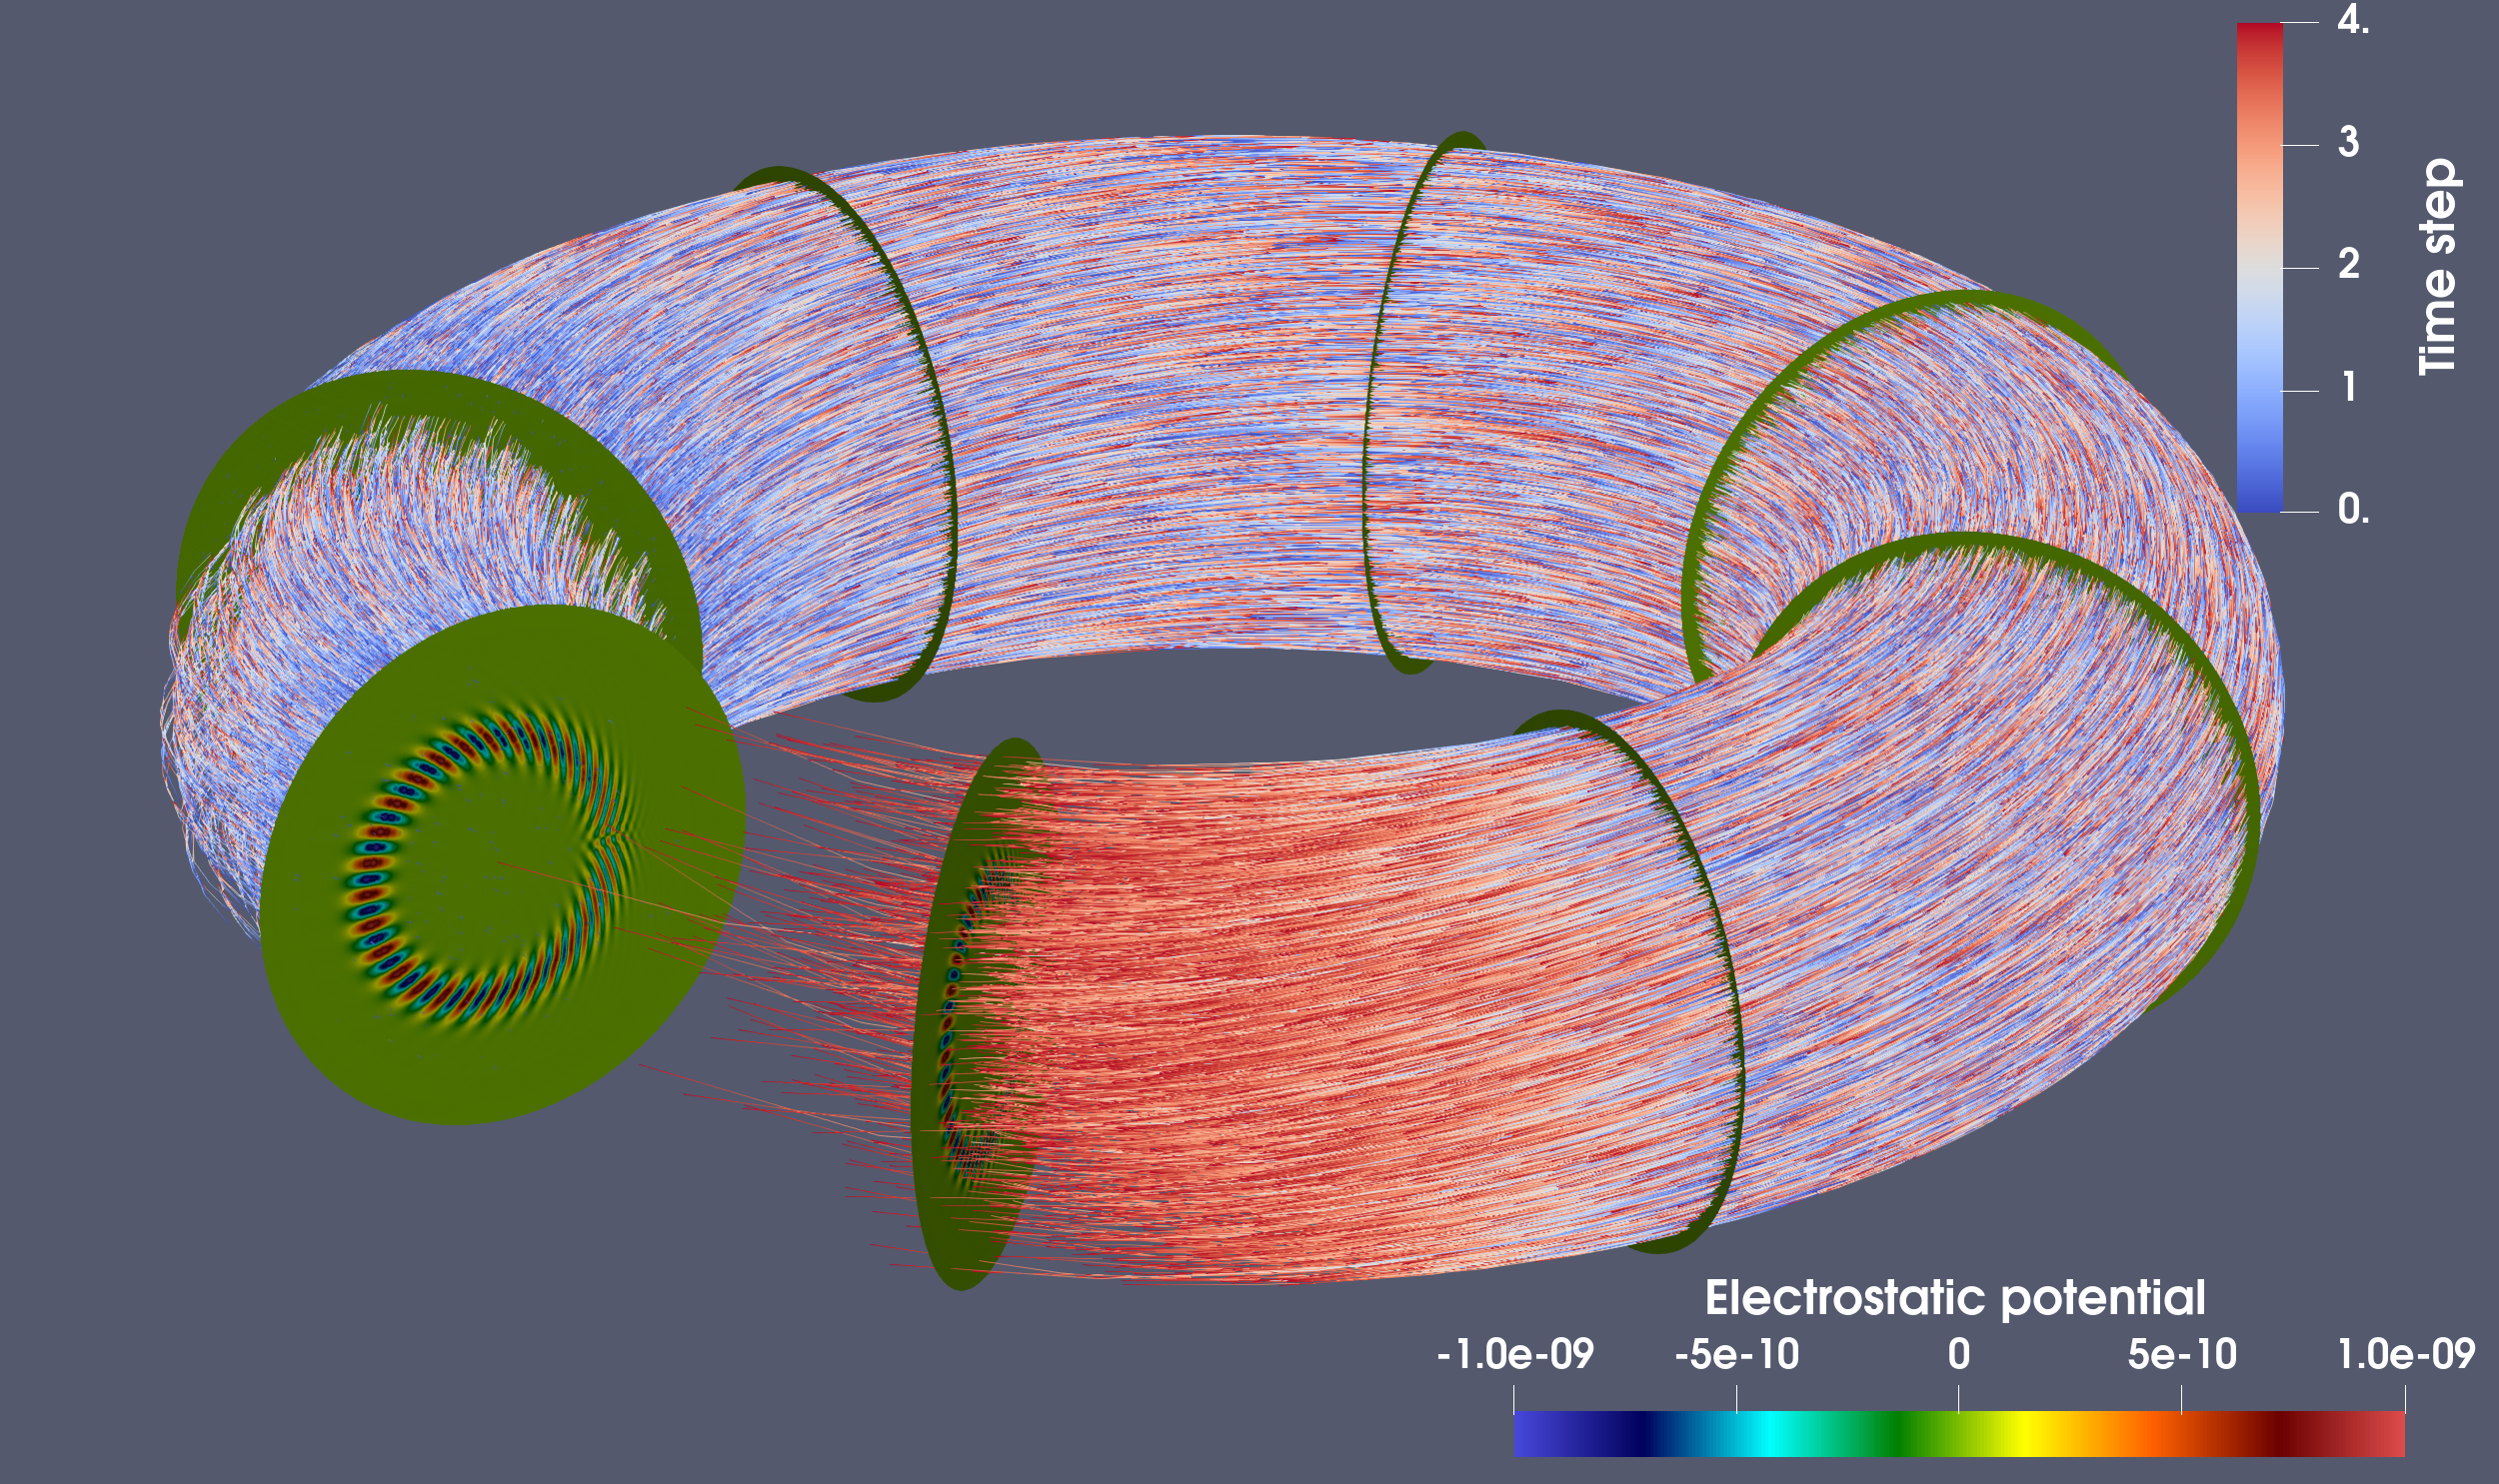
\includegraphics[height=.3\textheight]{cyclone_590k_30kptcls.png}
        \caption*{Eight planes depicted around the toroidal dimension}
      \end{figure}
    \end{column}
  \end{columns}
\end{frame}

%How EnGPar can be applied
\begin{frame}
  \frametitle{Applying EnGPar in XGC}
  \begin{itemize}
  \item Goal:
    \begin{itemize}
    \item Improve the load balancing in XGC using EnGPar.
    \item Provide a general approach to load balancing for future improvements.
    \end{itemize}
  \item Given the 1D partition of the mesh, the N-graph is defined as:
    \begin{itemize}
    \item One graph vertex for each mesh vertex.
    \item Graph edges connect mesh vertices with adjacent indices.
    \end{itemize}
  \item The weights computed by XGC for the ions, electrons and the collision operator are used as three different criteria to be balanced in EnGPar.
  \end{itemize}
\end{frame}

%Summary Slide
\begin{frame}
  \frametitle{Closing Remarks}
  \begin{itemize}
  \item EnGPar provides dynamic diffusive load balancing for a range of applications that can be represented by a hypergraph.
  \item We applied EnGPar to  improve imbalances of lower dimensional mesh entities of $>50\%$ for high-order unstructured mesh examples.
  \item EnGPar can reduce and maintain particle imbalances in mesh-based particle-in-cell simulations.
  \end{itemize}
  \textbf{Future Work}
  \begin{itemize}
  \item Compare EnGPar to the current load balancing method in XGC
    \begin{itemize}
    \item Explore further options in improving XGC's partition.
    \end{itemize}
  \item Increase the size and scale of current examples to see how these approaches perform.
  \item Apply EnGPar to other simulations and domains.
  \end{itemize}
\end{frame}
%Thank you slide
\begin{frame}
  \begin{columns}
    \begin{column}{.33\linewidth}
      \begin{figure}
        \centering
        
\includegraphics[width=\linewidth]{fastmath_logo.png}
      \end{figure}
    \end{column}
    \begin{column}{.33\linewidth}
      \begin{center}
        {\huge
          Thank You\\
          \bigskip
          \bigskip
          Questions?\\
          \bigskip
        }
      \end{center}
    \end{column}
    \begin{column}{.33\linewidth}
      \begin{figure}
        \centering
        
\includegraphics[width=\linewidth]{hbps_logo.png}
      \end{figure}
    \end{column}
  \end{columns}
  \vspace{.3cm}
  Part of the SciDAC supported project, ``Unstructured Mesh Technologies for Fusion Simulation Codes'' \\
  In collaboration with:
  \begin{itemize}
  \item FASTMath SciDAC Institute
  \item High-Fidelity Boundary Plasma Simulation SciDAC Partnership
  \item Plasma Surface Interactions SciDAC Partnership
  \item COPA: ECP Co-Design Center for Particle Applications
  \end{itemize}
\end{frame}

\end{document}
